\documentclass{beamer}
\usepackage{amsmath}
\usepackage{amsfonts}
\usepackage{amssymb}
\usepackage{natbib}
%\usepackage{fancyhdr}
%\usepackage[margin=1in]{geometry}
%%\usepackage{graphicx}
%%\usepackage{cite}
%%\usepackage{multicol}
%%\usepackage[section]{placeins}
%%\usepackage{amsthm}
\usepackage{nicefrac}
\usepackage{bm}
%%\usepackage{algorithm2e}
%\newtheorem{theorem}{Theorem}
%\newtheorem*{theorem*}{Theorem}
%\newtheorem{lemma}{Lemma}
%\newtheorem*{lemma*}{Lemma}
%\newtheorem*{def*}{Definition}
%\newtheorem*{conj}{Conjecture}
%\newtheorem{defn}{Definition}
%\newcommand{\low}[1]{$_{\text{#1}}$}
%\newcommand\xput[2][0.5]{%
%    \rule{#1\linewidth}{0pt}\makebox[0pt][c]{#2}\hfill}
%\usepackage{stackengine}
%\usepackage{enumerate}
\usepackage{tikz}
\usetikzlibrary{arrows.meta}
\usepackage{graphicx}
\usepackage{caption}
\usepackage{subcaption}

%
%\newcommand{\delt}[1]{
%\begin{tikzpicture}[#1]
%\draw (0,0) -- (1ex,1.5ex);
%\draw (2.1ex,0) -- (1ex,1.5ex);
%\draw (0.0,0.0) -- (2.1ex,0);
%\draw (0.5ex,0.8ex) -- (1.5ex, 0.8ex);
%\draw (1ex, 0.75ex) -- (1ex, 0);
%\end{tikzpicture}
%}
\usepackage[all]{xy}

\newcommand{\fp}{\varrho}
\newcommand{\nhalf}{\nicefrac{1}{2}}
%\newcommand{\eps}{\epsilon_{machine}}
\newcommand{\ol}{\overline}
\renewcommand{\b}{\bm}
%\newcommand{\problem}[2]{ \ \\\textbf{#1} \textit{#2}\\} 
%
\newcommand{\bE}{\mathbb{E}}
\newcommand{\bP}{\mathbb{P}}
\newcommand{\bR}{\mathbb{R}}
\newcommand{\bN}{\mathbb{N}}
\newcommand{\bZ}{\mathbb{Z}}
\newcommand{\bQ}{\mathbb{Q}}
\newcommand{\bC}{\mathbb{C}}
\newcommand{\cA}{\mathcal{A}}
\newcommand{\cB}{\mathcal{B}}
\newcommand{\cC}{\mathcal{C}}
\newcommand{\cD}{\mathcal{D}}
\newcommand{\cE}{\mathcal{E}}
\newcommand{\cF}{\mathcal{F}}
\newcommand{\cG}{\mathcal{G}}
\newcommand{\cH}{\mathcal{H}}
\newcommand{\cI}{\mathcal{I}}
\newcommand{\cJ}{\mathcal{J}}
\newcommand{\cK}{\mathcal{K}}
\newcommand{\cL}{\mathcal{L}}
\newcommand{\cM}{\mathcal{M}}
\newcommand{\cN}{\mathcal{N}}
\newcommand{\cO}{\mathcal{O}}
\newcommand{\cP}{\mathcal{P}}
\newcommand{\cQ}{\mathcal{Q}}
\newcommand{\cR}{\mathcal{R}}
\newcommand{\cS}{\mathcal{S}}
\newcommand{\cT}{\mathcal{T}}
\newcommand{\cU}{\mathcal{U}}
\newcommand{\cV}{\mathcal{V}}
\newcommand{\cW}{\mathcal{W}}
\newcommand{\cX}{\mathcal{X}}
\newcommand{\cY}{\mathcal{Y}}
\newcommand{\cZ}{\mathcal{Z}}

\definecolor{lblue}{RGB}{51,255,255}
\definecolor{dgreen}{RGB}{49,128,23}
\definecolor{nicepink}{RGB}{255, 0, 102}
\definecolor{nicered}{RGB}{255, 80, 80}

\newcommand{\kr}{\text{k}}
%
%\renewcommand{\arraystretch}{1.5}
%\renewcommand{\thefootnote}{\fnsymbol{footnote}}	
%\setlength{\headheight}{5pt}
%\pagestyle{fancyplain}
%\renewcommand{\headrulewidth}{0pt}
%\lhead{}
%\chead{}
%\rhead{}

%\lfoot{}
%\cfoot{\thepage}
%\rfoot{}

\setbeamerfont{block body}{size=\small}

\usetheme{Ilmenau}
\usecolortheme{seahorse}
\usefonttheme{serif}

\addtobeamertemplate{navigation symbols}{}{%
    \usebeamerfont{footline}%
    \usebeamercolor[fg]{footline}%
    \hspace{1em}%
    \insertframenumber/\inserttotalframenumber
}

\author[Brunner]{Jim Brunner}
\institute[LANL]{Los Alamos National Laboratory}
\title{Using Cooccurrance Networks}
\date{}
\begin{document}
%--------------------------------------------------------------------------------------------------
\begin{frame}
\titlepage
%\phantom{\cite{}}
\end{frame}
%--------------------------------------------------------------------------------------------------
\begin{frame}
\frametitle{Coincidence Network}
Constructing a coincidence network.
I map the abundances according to
\[
a(r_{ji})  = \left\{
\begin{array}{c c}
\lfloor\left(\frac{r_{ji}}{\max_{s_k}(r_{jk})}\right) n \rfloor + 1 &  \frac{r_{ji}}{\max_{s_k}(r_{jk})} \geq m \\
0 & \frac{r_{ji}}{\max_{s_k}(r_{jk})} < m
\end{array}
\right.
\]
into ``bins" relative to the maximum that taxa appears. Then count 
\[
w^1_{jk} = \frac{\|\{i: a(r_{ji}) = a(r_{ki}) \neq 0\} \|}{S}
\]
how often two organisms appear in the same bin.
\end{frame}
%--------------------------------------------------------------------------------------------------
%--------------------------------------------------------------------------------------------------
\begin{frame}
\frametitle{Cooccurrance Network}
Same idea but now edges weights are compared to a random graph (null model). 
\[
w_{jk}^2 = \left\{ \begin{array}{c c}
1 & P(w_{jk}^N \geq w_{jk}^1) \leq t\\
0 & P(w_{jk}^N < w_{jk}^1) > t
\end{array}\right.
\]
So we only keep edges that have a higher than ``random" weight.
\end{frame}
%--------------------------------------------------------------------------------------------------
%--------------------------------------------------------------------------------------------------
\begin{frame}
\frametitle{Using a Network}
\begin{itemize}
	\item Filter GOTTCHA results - try to determine probability of seeing groups of organisms - Random Markov Field
	\item Compare networks in different situations (clustering, connectivity, etc)
\end{itemize}
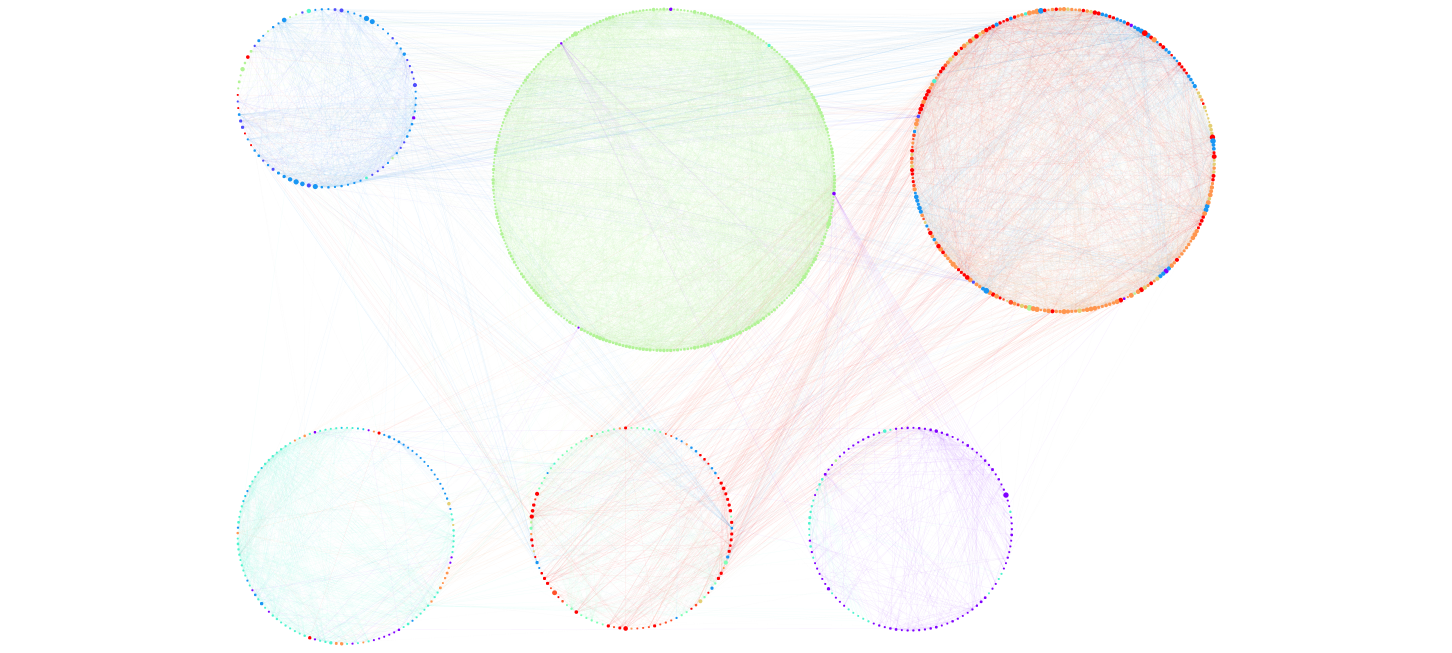
\includegraphics[scale = 0.2]{june20/june20_species.png}

\end{frame}
%--------------------------------------------------------------------------------------------------
%\begin{frame}
%\frametitle{References}
%\bibliographystyle{unsrt}
%% make bibliography entries smaller
%\renewcommand\bibfont{\scriptsize}
%% and kill the abominable icon
%\setbeamertemplate{bibliography item}{}
%\bibliography{summer17}
%\end{frame}
%%--------------------------------------------------------------------------------------------------
%--------------------------------------------------------------------------------------------------
%\begin{frame}
%\frametitle{Thank You}
%
%
%\end{frame}
%%--------------------------------------------------------------------------------------------------
\end{document}